% Created 2025-03-28 sex 09:49
% Intended LaTeX compiler: pdflatex
\documentclass[11pt]{article}
\usepackage[utf8]{inputenc}
\usepackage[T1]{fontenc}
\usepackage{graphicx}
\usepackage{longtable}
\usepackage{wrapfig}
\usepackage{rotating}
\usepackage[normalem]{ulem}
\usepackage{amsmath}
\usepackage{amssymb}
\usepackage{capt-of}
\usepackage{hyperref}
\author{jo}
\date{\today}
\title{}
\hypersetup{
 pdfauthor={jo},
 pdftitle={},
 pdfkeywords={},
 pdfsubject={},
 pdfcreator={Emacs 27.1 (Org mode 9.7.20)}, 
 pdflang={English}}
\begin{document}

\tableofcontents

\section{Pré-física}
\label{sec:org2f323eb}

\subsection{Grandezas e Unidades de Medida}
\label{sec:org8ef5ce4}

As grandezas físicas são conceitos aos quais podemos atribuir valores
numéricos, enquanto que as unidades de medida são padrões de medida
para cada grandeza correspondente.


Na tabela abaixo estão algumas grandezas físicas com correspondentes unidades de medida:

\begin{table}[htbp]
\caption{Grandezas e unidades de medida.}
\centering
\begin{tabular}{lll}
Grandeza & Unidade (Nome) & Unidade (Símbolo)\\
\hline
Massa & Quilograma, Grama & kg, g\\
Volume & Litro, Mili-litro & L, mL\\
Densidade & Grama por mili-litro & g/mL\\
Comprimento & Metro, Centímetro & m, cm\\
Tempo & Hora, Segundo & h, s\\
\end{tabular}
\end{table}

\href{quest-pre-fisica1.org}{Questões de Revisão: Grandezas e Unidades de Medida} 
\subsection{Equações}
\label{sec:orgee1bef8}
As equações na física são relações matemáticas entre
grandezas. Considere os seguintes dados de uma substância hipotética:

\begin{table}[htbp]
\caption{Massa, volume e densidade}
\centering
\begin{tabular}{lll}
Massa (g) & Volume (mL) & Densidade (g/mL)\\
\hline
3,0 & 1,0 & 3,0\\
6,0 & 2,0 & 3,0\\
\(?\) & 2,5 & 3,0\\
10,5 & \(?\) & 3,0\\
15,0 & 5,0 & \(?\)\\
\end{tabular}
\end{table}



A densidade é calculada dividindo a massa pelo volume. Essa relação pode ser escrita como:

\begin{equation}
d = \frac{m}{V}
\end{equation}

Onde:
\begin{itemize}
\item \(m\) = massa
\item \(V\) = volume
\item \(d\) = densidade
\end{itemize}

Com dois valores conhecidos, podemos calcular o terceiro.

\href{quest-pre-fisica2.org}{Questões de revisão: equações}
\subsection{Gráficos}
\label{sec:org98f015b}
Gráficos são ferramentas visuais importantes para representar dados e relações entre grandezas físicas. Eles ajudam a identificar padrões e tendências.


Como exemplo, os dados abaixo,

\begin{table}[htbp]
\caption{Massa e volume de uma substância hipotética}
\centering
\begin{tabular}{ll}
Volume (mL) & Massa (g)\\
\hline
1,0 & 3,0\\
2,0 & 6,0\\
3,0 & 9,0\\
4,0 & 12,0\\
5,0 & 15,0\\
\end{tabular}
\end{table}

Podem ser representados pela figura

\begin{figure}[htbp]
\centering
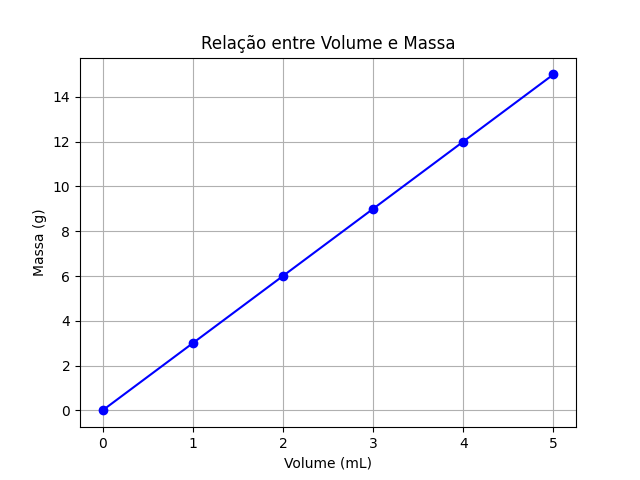
\includegraphics[width=.9\linewidth]{graphics/grafico1.png}
\caption{Gráfico que relaciona os valores de massa e volume da tabela anterior.}
\end{figure}

\href{quest-pre-fisica3.org}{Questões de revisão: gráficos} 
\end{document}
